%%%%%%%%%%%%%%%%%%%%%%%%%%%%%%%%%%%%%%%%%%%%%%%%%%%%%%%%%%%%%%%%%%%
%                                                                 %
%                            CHAPTER SIX                          %
%                                                                 %
%%%%%%%%%%%%%%%%%%%%%%%%%%%%%%%%%%%%%%%%%%%%%%%%%%%%%%%%%%%%%%%%%%%

\chapter{MBVL CLASSIFICATION}\label{ch:mbvl}

The goal of this section is to use the versioning graph to compare the accuracy of different algorithm and taxonomy combinations in determining the taxonomic classification of marine microbiological species.

\section{Versioning Graph}

The experiment undergoes two phases of comparison in this procedure.
The first phase compares the initial species content with the classifications by a particular algorithm/taxonomy combination.
Since the classification results from a population selected according to the initial species list, these two data sets share a common provenance.
However, the list cannot be used in place of the classifier results because not only does it have only 21 entries, but also it does not have a clear correspondence with the DNA chains sent to the classifier.
As a result, these two sets are not versions of each other, and versioning results will have weak implications.
A labeling of the initial input data, could be considered a version of the results, but that data product is not available.

Each taxonomy and classifier combination outputs a taxonomic classification for each entry from the same source.
Shared input data indicates the results share common provenance.
The classifications also share the same workflow step because their results have similar formats, reporting a specific taxonomic name for each entry.
Since classifications occur over the same set of entries, their identifiers can be used to match outputs together for comparison.
However, if this method of matching is used, every mapping would be a modification since each identifier appears in all data sets, and it would not provide any comparison based on the algorithm's specificity.
Instead, a mapping using the accuracy of each algorithm is used.
Since a name is assigned at a taxonomic rank to a sequence only if it passes the algorithm's confidence level, matches can be determined on whether a classifier can confidently decide more or fewer ranks.
As a result, additions and invalidations ascertain whether a classifier can identify more or less of an entry's taxonomic name while modifications indicate the same specificity but mismatching names.
This method of mapping versions allows the results to give insight into the accuracy of different algorithm and taxonomy combinations.

\section{Analysis}

Figure \ref{mbvl_chart} shows the results of four comparisons performed using the matching procedure in the previous section.
There are only four comparisons because varying both taxonomy and algorithm muddles the contribution of each towards a more accurate result.
In the first set of columns, the Silva taxonomy results are versioned against RDP using the Spingo algorithm.
The naming reflects the orientation in the versioning graph so Silva forms the left-hand version and RDP would be the right-hand version.
In this comparison, using the RDP taxonomy seems to provide more accurate results, most specifically at the species level.
The taxonomies also disagree fairly often at the species and family ranks.
Switching to the Gast algorithm in the second set of columns, RDP once again demonstrates a noticeably greater accuracy in species classification.
There are also significantly fewer disagreements using the Gast algorithm between the two taxonomies.
Looking at the third set of columns, Silva demonstrates greater accuracy classifications under the Spingo algorithm than under Gast.
Over four thousand of these entries can be classified to the species level when Gast cannot.
In the fourth set of columns, RDP appears to perform better with Spingo than Gast.
However, the comparison is dominated by a much larger number of disagreements between almost six thousand entries, primarily at the species rank.
On closer inspection, this disagreement is explained by Gast classifying the species for a number of entries as unclutured bacterium.
This analysis presents evidence that using the RDP taxonomy with the Spingo algorithm will produce the most accurate classification results.

\begin{figure}
	\centering
	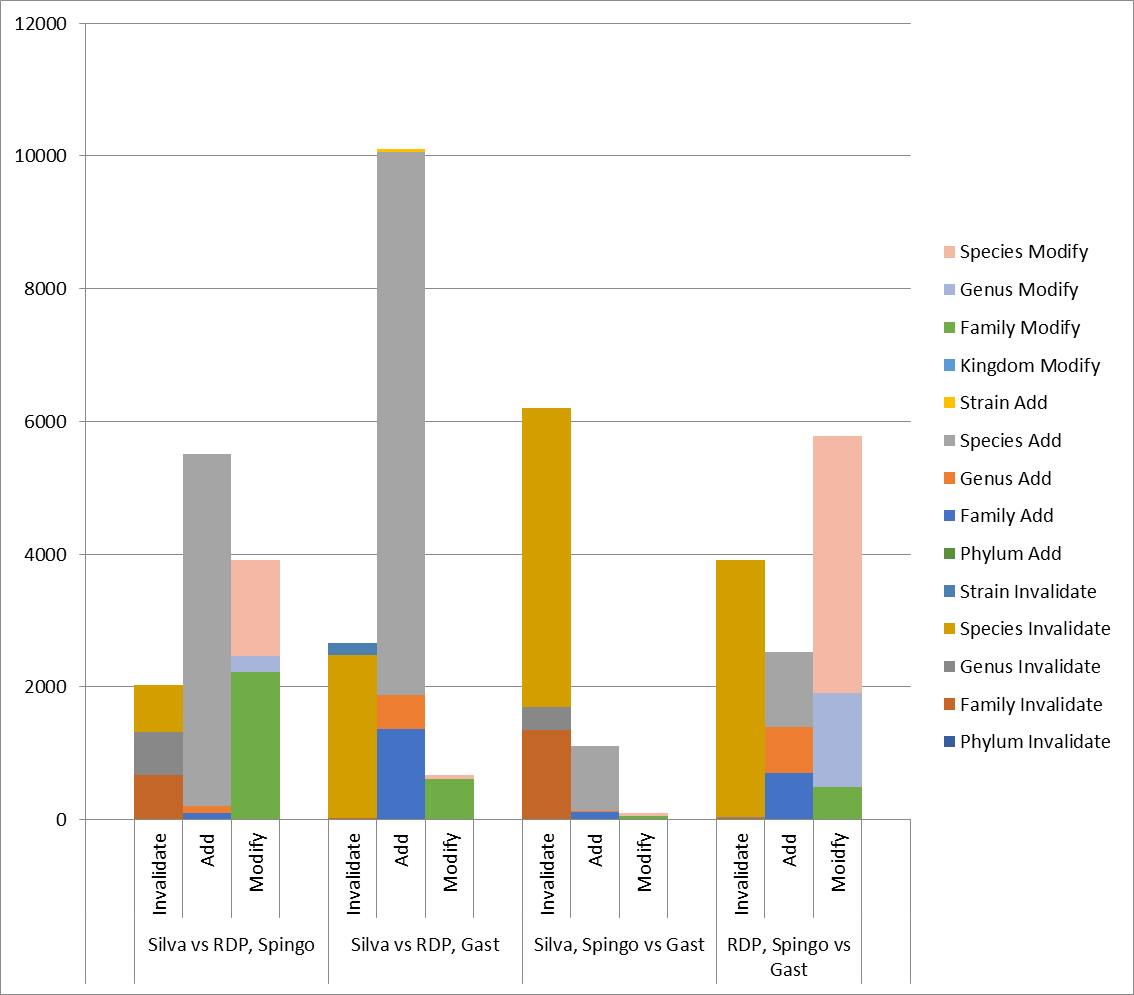
\includegraphics[scale=0.80]{figures/mbvl_chart.png}
	\caption{Compiled counts of adds, invalidates, and modifies grouped by taxonomic rank across algorithm and taxonomy combinations.}
	\label{mbvl_chart}
\end{figure}